\documentclass[10pt,letterpaper,notumble]{leaflet}

\usepackage[T1]{fontenc}
\usepackage[utf8]{inputenc}
\usepackage{listingsutf8}
\usepackage[spanish]{babel}
\usepackage{microtype}
\usepackage{blindtext} 
\usepackage{biolinum} 
\renewcommand\rmdefault{\sfdefault}% Verwende serifenlose Schrift 
\usepackage{mwe}% Dummy Bilder 
\usepackage{graphicx}
\usepackage{verbatim}
\usepackage{xcolor}
	\definecolor{WildStrawberry}{rgb}{1.0, 0.26, 0.64}
	\definecolor{wildstrawberry}{rgb}{1.0, 0.26, 0.64}
	\definecolor{Mulberry}{rgb}{0.77, 0.29, 0.55}
	\definecolor{LimeGreen}{rgb}{0.2, 0.8, 0.2}
	\definecolor{LincolnGreen}{rgb}{0.11, 0.35, 0.02}
	\definecolor{blue}{rgb}{0.0, 0.0, 1.0}
	\definecolor{forestgreen(traditional)}{rgb}{0.0, 0.27, 0.13}
\usepackage[colorlinks,citecolor=blue,urlcolor=blue]{hyperref}


\AddToBackground{5}{\put(0,0){\textcolor{blue!5}{\rule{\paperwidth}{\paperheight}}}}%

\AddToBackground{5}{% Fondo de la página pequeña 1
	\put(\LenToUnit{0.05\paperwidth},\LenToUnit{0.875\paperheight}){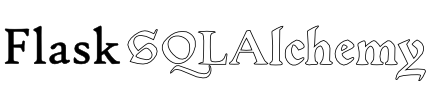
\includegraphics[width=\LenToUnit{0.90\paperwidth},height=\LenToUnit{0.1\paperheight}]{../img/flask-sqlalchemy-title.png}}
}

\title{Quik Reference} 
\author{Ferreira Juan David} 
\date{\today} % Experiment 1

\AddToBackground{5}{% Fondo de la página pequeña 1
	\put(\LenToUnit{0.05\paperwidth},\LenToUnit{0.05\paperheight}){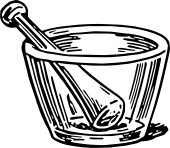
\includegraphics[width=\LenToUnit{0.75\paperwidth},height=\LenToUnit{0.25\paperheight}]{../img/flask-sqlalchemy-logo.png}}
}

\AddToBackground{4}{\put(0,0){\textcolor{blue!5}{\rule{\paperwidth}{\paperheight}}}}%

\begin{document}
	\mbox{}
	\thispagestyle{empty}% Keine Seitenzahlen 
	
	\clearpage
	\makebox[\linewidth][l]{
		\begin{minipage}{2.2\linewidth}
		    
			Dado que una persona sin nombre o una dirección de correo electrónico sin dirección asociada no tiene sentido, \texttt{nullable=False} le dice a \texttt{SQLAlchemy} que cree la columna como \texttt{NOT NULL}. Esto está implícito para las columnas de clave \textit{primaria}, pero es una buena práctica especificarlo para todas las demás columnas, para que dejemos en claro a otras personas que trabajan en nuestro código que realmente deseaba una columna \texttt{NULL} y no fue simplemente que se nos olvidó de agregarla.
						
			Entonces, ¿qué significan \texttt{\textcolor{forestgreen(traditional)}{backref}} y \texttt{\textcolor{forestgreen(traditional)}{lazy}}?. \texttt{\textcolor{forestgreen(traditional)}{backref}} es una forma sencilla de declarar también una nueva propiedad en la clase \texttt{Address}. A continuación, también puede utilizar \texttt{my\_address.person} para llegar a la persona en esa dirección. \texttt{\textcolor{forestgreen(traditional)}{lazy}} define cuándo \texttt{SQLAlchemy} cargará los datos de la base de datos:
			
			\begin{itemize}
				\item \texttt{'select'/True} (es el valor por default, pero dejarlo explícito es mejor que implícito) significa que \texttt{SQLAlchemy} cargará los datos según sea necesario de una sola vez utilizando una declaración \texttt{SELECT} estándar.
				
				\item \texttt{'joined'/False} le dice a \texttt{SQLAlchemy} que cargue la relación en la misma consulta que el padre usando una declaración \texttt{JOIN}.
				
				\item \texttt{'subquery'} funciona como \texttt{'joined'} pero en su lugar \texttt{SQLAlchemy} usará una subconsulta.
				
				\item \texttt{'dynamic'} es especial y puede resultar útil si tiene muchos elementos y siempre desea aplicarles filtros \texttt{SQL} adicionales. En lugar de cargar los elementos, \texttt{SQLAlchemy} devolverá otro objeto de consulta que puede refinar aún más antes de cargar los elementos. Tengamos en cuenta que esto no se puede convertir en una estrategia de carga diferente al realizar consultas, por lo que a menudo es una buena idea evitar usar esto a favor de \texttt{lazy=True}.Se puede crear un objeto de consulta equivalente a una relación dinámica \texttt{user.address} usando \texttt{Address.query.with\_parent(user)} mientras se puede usar la carga diferida o ansiosa en la relación en sí, según sea necesario.
			\end{itemize}
			
			¿Cómo se define el \texttt{lazy status} para \texttt{backrefs}?. Usando la función \texttt{backref()}:
			
			\lstset{inputencoding=utf8/latin1,
				frame=lines,
				label={lst:code_direct},
				basicstyle=\footnotesize,
				showstringspaces=false  
			}
			\lstinputlisting[language=Python,firstline=20,lastline=24]{../python/03-models.py}	
			
			\vspace*{-0.6cm}
			
			\section{Relación muchos a muchos}
			
			Si desea utilizar relaciones de varios a varios, deberá definir una tabla auxiliar que se utilice para la relación. Para esta mesa auxiliar, se recomienda encarecidamente no utilizar un modelo, sino una mesa real:
			
			
			\lstinputlisting[language=Python,firstline=26,lastline=37]{../python/03-models.py}
			
			Aquí configuramos \texttt{Page.tags} para que se cargue inmediatamente después de cargar una página, pero usando una consulta separada. Esto siempre da como resultado dos consultas al recuperar una página, pero al consultar varias páginas no obtendrá consultas adicionales.
			
		\end{minipage}
		
	}

    \clearpage
    
    \mbox{}
    
	\clearpage % end the column
	
	La lista de páginas para una etiqueta, por otro lado, es algo que rara vez se necesita. Por ejemplo, no necesitará esa lista al recuperar las etiquetas de una página específica. Por lo tanto, el \texttt{backref} está configurado para cargarse de forma diferida, de modo que acceder a él por primera vez desencadenará una consulta para obtener la lista de páginas para esa etiqueta. Si necesita aplicar más opciones de consulta en esa lista, puede cambiar a la estrategia \texttt{'dynamic'}, con los inconvenientes mencionados anteriormente, u obtener un objeto de consulta \texttt{Page.query.with\_parent(some\_tag)} y luego usarlo exactamente como lo haría con el objeto de consulta de una relación dinámica.
	
	\clearpage % end the spanned column
	
	\maketitle
	
	\begin{abstract}
		Generalmente, \texttt{Flask-SQLAlchemy} se comporta como una base declarativa configurada correctamente desde la extensión declarativa. Como tal, recomendamos leer los documentos de \texttt{SQLAlchemy} para obtener una referencia completa. Sin embargo, los casos de uso más comunes también se documentan aquí.
		
		\textbf{Cosas a tener en cuenta:}
		
		\begin{itemize}
			\item La clase base para todos sus modelos se llama \texttt{db.Model}. Se almacena en la instancia de \texttt{SQLAlchemy} que debe crear. Consulte Inicio rápido para obtener más detalles.
			
			\item Algunas partes que se requieren en \texttt{SQLAlchemy} son opcionales en \texttt{Flask-SQLAlchemy}. Por ejemplo, el nombre de la tabla se establece automáticamente a menos que se anule. Se deriva del nombre de la clase convertido a minúsculas y con ``\texttt{CamelCase}'' convertido a ``\texttt{camel\_case}''. Para anular el nombre de la tabla, establezca el atributo \texttt{\_\_tablename\_\_} de clase.
		\end{itemize}
	\end{abstract}
	
	\thispagestyle{empty}
	
	\clearpage
	\makebox[\linewidth][l]{
		\begin{minipage}{2.2\linewidth}
			
			\section{Declaración de modelos}
			
			\lstset{inputencoding=utf8/latin1,
				frame=lines,
				label={lst:code_direct},
				basicstyle=\footnotesize,
				showstringspaces=false  
			}
			\lstinputlisting[language=Python,firstline=1,lastline=7]{../python/03-models.py}
			
			Usamos \texttt{Column} para definir una columna. El nombre de la columna es el nombre que le asigna. Si desea utilizar un nombre diferente en la tabla, puede proporcionar un primer argumento opcional que es una cadena con el nombre de columna deseado. Las claves primarias están marcadas con \texttt{primary\_key=True}. Se pueden marcar varias claves como claves primarias, en cuyo caso se convierten en una clave primaria compuesta.
			
			Los tipos de columna son el primer argumento de \texttt{Column}. Puede proporcionarlos directamente o llamarlos para especificarlos más (como proporcionar una longitud). Los siguientes tipos son los más comunes:
			
			\begin{description} 
				\item[\texttt{Integer}:]
				Un entero. 
				\item[\texttt{String(size)}:]
				Una cadena con una longitud máxima (opcional en algunas bases de datos, por ejemplo, \texttt{PostgreSQL}).
				\item[\texttt{Text}:] 
				Algo de texto Unicode más largo.
				\item[\texttt{DateTime}:] 
				Fecha y hora expresadas como objeto \texttt{datetime} de \texttt{Python}.
				\item[\texttt{Float}:]
				Almacena valores de coma flotante.
				\item[\texttt{Boolean}:]
				Almacena un valor booleano.
				\item[\texttt{PickleType}:] \textcolor{red}{Corregir}
%				Almacena un objeto \texttt{Python} en escabeche.
				\item[\texttt{LargeBinary}:]
				Almacena grandes datos binarios arbitrarios.
			\end{description}
		
		    \section{Relaciones One-to-Many}
		    
		    Las relaciones más comunes son las relaciones de uno a varios. Debido a que las relaciones se declaran antes de que se establezcan, puede usar cadenas para hacer referencia a clases que aún no se han creado (por ejemplo, si \texttt{Person} define una relación a \texttt{Address} que se declara más adelante en el archivo).
		    
		    Las relaciones se expresan con la función \texttt{\textcolor{blue}{relationship()}}. Sin embargo, la clave \textit{foránea} debe declararse por separado con la clase \texttt{ForeignKey}:
		    
		    \lstinputlisting[language=Python,firstline=9,lastline=17]{../python/03-models.py}
		    
		    ¿Qué \texttt{\textcolor{blue}{db.relationship()}} utilizar?. Esa función devuelve una nueva propiedad que puede hacer varias cosas. En este caso, le dijimos que apunte a la clase \texttt{Address} y cargue varios de ellos. \textit{¿Cómo sabemos que esto devolverá más de una dirección?}. Porque \texttt{SQLAlchemy} adivina un valor predeterminado útil de su declaración. Si queremos tener una relación uno-a-uno puede pasar el parámetro \texttt{uselist=False} a \texttt{\textcolor{blue}{relationship()}}.
		\end{minipage}
		
	}
	
\end{document}